\documentclass[tikz,border=0pt]{standalone}
\usepackage{xcolor}
\usetikzlibrary{calc}
% Palette: Sam_Comm_final.png by eye, and the drones and raiders.
\definecolor{ink}{HTML}{3B2340}
\definecolor{sky}{HTML}{EFC46A}
\definecolor{skyhi}{HTML}{F5DA92}
\definecolor{skylow}{HTML}{E9B060}
\definecolor{cloud}{HTML}{F2D58A}
\definecolor{paper}{HTML}{FBEFD0}
\definecolor{cream}{HTML}{FFF6E0}
\definecolor{white}{HTML}{FFFFFF}
\definecolor{wallA}{HTML}{E88A73}
\definecolor{wallB}{HTML}{EE9F7E}
\definecolor{wallC}{HTML}{E47A7E}
\definecolor{wallD}{HTML}{F0B07E}
\definecolor{wallE}{HTML}{D9765F}
\definecolor{wallF}{HTML}{E99A8A}
\definecolor{greenA}{HTML}{8DBB7E}
\definecolor{greenB}{HTML}{6FA77A}
\definecolor{greenC}{HTML}{A9C97F}
\definecolor{greenD}{HTML}{5E9C6A}
\definecolor{greenE}{HTML}{4A8060}
\definecolor{sage}{HTML}{9DB98A}
\definecolor{sagedark}{HTML}{6F8F66}
\definecolor{sagelight}{HTML}{C2D6A6}
\definecolor{window}{HTML}{F6E7A0}
\definecolor{windark}{HTML}{8C5A64}
\definecolor{metal}{HTML}{8D9A93}
\definecolor{metaldark}{HTML}{5E6B66}
\definecolor{metallight}{HTML}{B9C4BC}
\definecolor{wood}{HTML}{B9835A}
\definecolor{wooddark}{HTML}{8C5A3C}
\definecolor{woodlight}{HTML}{D9A66F}
\definecolor{stone}{HTML}{E7C9A0}
\definecolor{stonedark}{HTML}{C9A47E}
\definecolor{concrete}{HTML}{D8C3A4}
\definecolor{concretedark}{HTML}{B8A084}
\definecolor{asphalt}{HTML}{8E7A86}
\definecolor{asphaltdark}{HTML}{6E5C68}
\definecolor{roadline}{HTML}{F6E7A0}
\definecolor{kerb}{HTML}{D8B48C}
\definecolor{red}{HTML}{E0483E}
\definecolor{redlight}{HTML}{F27A6A}
\definecolor{gold}{HTML}{FFB000}
\definecolor{goldlight}{HTML}{FFD54F}
\definecolor{teal}{HTML}{4FA3A0}
\definecolor{tealdark}{HTML}{3C8582}
\definecolor{magenta}{HTML}{FF2E88}
\definecolor{cyan}{HTML}{13CFE3}
\definecolor{violet}{HTML}{8A5BD6}
\definecolor{orange}{HTML}{F2803A}
\definecolor{pink}{HTML}{F48FB1}
\definecolor{glow}{HTML}{4FE6E0}
\definecolor{glowhi}{HTML}{C8FFF9}
\definecolor{hot}{HTML}{FF6A1A}
\definecolor{hothi}{HTML}{FFD07A}
\definecolor{armour}{HTML}{7E7A86}
\definecolor{armourdark}{HTML}{5A5466}
\definecolor{armourlight}{HTML}{A8A2B0}
\definecolor{wasp}{HTML}{E0A82E}
\definecolor{waspdark}{HTML}{B07E1A}
\definecolor{moth}{HTML}{F2E6C8}
\definecolor{mothdark}{HTML}{D2C09A}
\definecolor{hornet}{HTML}{3C8582}
\definecolor{hornetdark}{HTML}{2C6260}
\definecolor{warden}{HTML}{E47A7E}
\definecolor{wardendark}{HTML}{B85A62}
\definecolor{tick}{HTML}{8DBB7E}
\definecolor{tickdark}{HTML}{5E8A5A}
\definecolor{strider}{HTML}{D9765F}
\definecolor{striderdark}{HTML}{A8543F}
\definecolor{jacket}{HTML}{6FA77A}
\definecolor{jacketb}{HTML}{4FA3A0}
\definecolor{jacketc}{HTML}{E88A73}
\definecolor{jacketd}{HTML}{F0B07E}
\definecolor{skin}{HTML}{F2C49A}
\definecolor{skinb}{HTML}{C98C6A}
\definecolor{skinc}{HTML}{8C5A3C}
\definecolor{hair}{HTML}{3B2340}
\definecolor{goo}{HTML}{B6E35A}
\definecolor{goodark}{HTML}{7FB23A}
\newcommand{\Ink}{1.8pt}
\tikzset{inked/.style={draw=ink, line width=\Ink, line join=round, line cap=round}}
\begin{document}
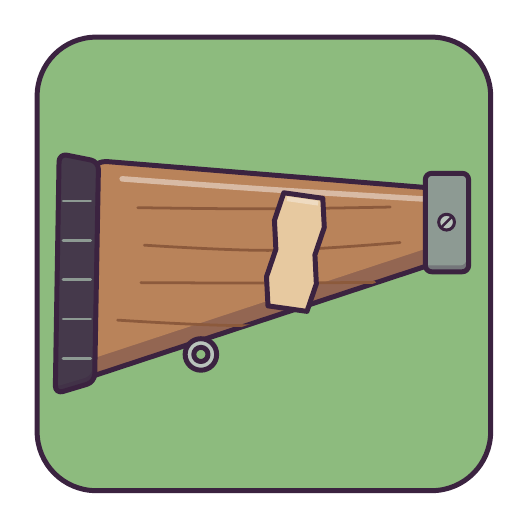
\begin{tikzpicture}
\clip (0,0) rectangle (6,6);
\fill[greenA] [rounded corners=0.75cm] (0.12,0.12) rectangle (5.88,5.88);
\begin{scope}\clip [rounded corners=0.75cm] (0.12,0.12) rectangle (5.88,5.88);
\begin{scope}\clip (5.3,3.95) -- (1.0,4.3) .. controls (0.85,4.3) and (0.8,4.2) .. (0.8,4.05) -- (0.75,1.55) -- (5.3,3.05) -- cycle;
\fill[wood!70!ink] (5.3,3.95) -- (1.0,4.3) .. controls (0.85,4.3) and (0.8,4.2) .. (0.8,4.05) -- (0.75,1.55) -- (5.3,3.05) -- cycle;
\fill[wood, shift={(-0.07,0.2)}] (5.3,3.95) -- (1.0,4.3) .. controls (0.85,4.3) and (0.8,4.2) .. (0.8,4.05) -- (0.75,1.55) -- (5.3,3.05) -- cycle;
\end{scope}
\draw[inked] (5.3,3.95) -- (1.0,4.3) .. controls (0.85,4.3) and (0.8,4.2) .. (0.8,4.05) -- (0.75,1.55) -- (5.3,3.05) -- cycle;
\begin{scope}\clip (5.3,3.95) -- (1.0,4.3) .. controls (0.85,4.3) and (0.8,4.2) .. (0.8,4.05) -- (0.75,1.55) -- (5.3,3.05) -- cycle;
\draw[wooddark, line width=1pt, line cap=round, line join=round] plot[smooth, tension=0.6] coordinates {(1.142,2.286) (2.844,2.216) (4.546,2.32)};
\draw[wooddark, line width=1pt, line cap=round, line join=round] plot[smooth, tension=0.6] coordinates {(1.439,2.762) (2.923,2.757) (4.406,2.765)};
\draw[wooddark, line width=1pt, line cap=round, line join=round] plot[smooth, tension=0.6] coordinates {(1.481,3.238) (3.105,3.172) (4.729,3.271)};
\draw[wooddark, line width=1pt, line cap=round, line join=round] plot[smooth, tension=0.6] coordinates {(1.398,3.714) (3.002,3.699) (4.605,3.722)};
\end{scope}
\draw[white, line width=2pt, line cap=round, line join=round, opacity=0.45] plot[smooth, tension=0.6] coordinates {(1.2,4.08) (3,3.95) (5.1,3.82)};
\begin{scope}\clip[rounded corners=0.1cm] (0.35,1.35) -- (0.85,1.5) -- (0.9,4.3) -- (0.4,4.4) -- cycle;
\fill[ink!70!metaldark!70!ink,rounded corners=0.1cm] (0.35,1.35) -- (0.85,1.5) -- (0.9,4.3) -- (0.4,4.4) -- cycle;
\fill[ink!70!metaldark,rounded corners=0.1cm, shift={(-0.028,0.08)}] (0.35,1.35) -- (0.85,1.5) -- (0.9,4.3) -- (0.4,4.4) -- cycle;
\end{scope}
\draw[inked,rounded corners=0.1cm] (0.35,1.35) -- (0.85,1.5) -- (0.9,4.3) -- (0.4,4.4) -- cycle;
\draw[metal, line width=1pt, line cap=round] (0.45,1.8) -- (0.8,1.8);
\draw[metal, line width=1pt, line cap=round] (0.45,2.3) -- (0.8,2.3);
\draw[metal, line width=1pt, line cap=round] (0.45,2.8) -- (0.8,2.8);
\draw[metal, line width=1pt, line cap=round] (0.45,3.3) -- (0.8,3.3);
\draw[metal, line width=1pt, line cap=round] (0.45,3.8) -- (0.8,3.8);
\begin{scope}\clip[rounded corners=0.08cm] (5.05,2.9) rectangle (5.6,4.15);
\fill[metal!70!ink,rounded corners=0.08cm] (5.05,2.9) rectangle (5.6,4.15);
\fill[metal,rounded corners=0.08cm, shift={(-0.028,0.08)}] (5.05,2.9) rectangle (5.6,4.15);
\end{scope}
\draw[inked,rounded corners=0.08cm] (5.05,2.9) rectangle (5.6,4.15);
\filldraw[inked,fill=metallight,line width=1.1pt] (5.32,3.53) circle (0.1);
\draw[ink, line width=0.9pt, line cap=round] (5.265,3.475) -- (5.375,3.585);
\filldraw[inked,fill=metallight] (2.2,1.85) circle (0.2);
\filldraw[inked,fill=greenA] (2.2,1.85) circle (0.09);
\filldraw[inked,fill=stone] (3.052,2.467) -- (3.547,2.397) -- (3.666,2.746) -- (3.648,3.115) -- (3.767,3.464) -- (3.748,3.833) -- (3.253,3.903) -- (3.134,3.554) -- (3.152,3.185) -- (3.033,2.836) -- cycle;
\fill[white, opacity=0.35] (3.289,3.797) -- (3.685,3.741) -- (3.693,3.8) -- (3.297,3.856) -- cycle;
\end{scope}
\draw[inked] [rounded corners=0.75cm] (0.12,0.12) rectangle (5.88,5.88);
\end{tikzpicture}
\end{document}
